\section{Experimental Setup}
\label{sec:setup}

\paragraph{Data}
We use the Millionbase dataset which is freely available and has close to 2.9 million quality chess games.\footnote{Download link available at \url{https://rebel13.nl/rebel13/rebel\%2013.html}}
After filtering out duplicate games, games with
fewer than 10 moves, and games with
more than 150 moves (for the complete game to fit into one transformer window), we are left with around 2.5 million games.
From this filtered set we randomly select 200K games for training, 15K games each for dev and test, and another 50K games to create board state probing evaluation sets described in Section~\ref{sec:cloze}.
The dev and test sets are used for perplexity evaluations. 
The dev set perplexity is used for choosing hyperparameters.
From the 200K training set, we create subsets of size 15K and 50K which we refer to as ``Train-S'' and ``Train-M'', while the full training set is referred to as ``Train-L''.
For detailed statistics, see Table~\ref{tab:data_stats} in Appendix.
All the data processing steps requiring chess knowledge, including parsing chess databases, are carried out using python-chess~\citep{python-chess}.

To create the board state probing evaluation sets, we use the 50K games reserved for this task. %
We only consider prompts for non-pawn pieces since the dynamics of pawns are fairly limited.
We ensure that the game prefixes selected are never seen in the training data.
The final evaluation set consists of 1000 instances with prefix length (in number of moves) in the range $51 \le l \le 100$.





\begin{figure*}
	\begin{minipage}{\textwidth}
		\begin{minipage}[b]{0.48\textwidth}
			\centering
			\begin{tabular}{llcc}
				\toprule
				Training Set & Model   & Dev set & Test set \\
				\midrule
				\multirow{2}{*}{Train-S} 
				& UCI 				& 23.6 & 23.6\\
				& UCI + RAP 		& 15.9 & 15.9\\
				& UCI + \piecetype 	& 16.1 & 16.2 \\
				\midrule
				\multirow{2}{*}{Train-M} 
				& UCI 				& 11.6 & 11.6\\
				& UCI + RAP 		& 10.4 & 10.4\\
				& UCI + \piecetype 	& 10.1 & 10.0 \\
				\midrule
				\multirow{2}{*}{Train-L} 
				& UCI 				& \phantom{1}7.7 & \phantom{1}7.7\\
				& UCI + RAP 		& \phantom{1}7.4 & \phantom{1}7.4\\
				& UCI + \piecetype 	& \phantom{1}7.2 & \phantom{1}7.2 \\
				\bottomrule
				
			\end{tabular}
			\captionof{table}{Canonical validation and test set perplexity. By canonical we mean that one move, say \pos{f1b5}, counts as one token.}
			\label{tab:perplexity}
		\end{minipage}
		\hfill
		\begin{minipage}[b]{0.48\textwidth}
			\centering
			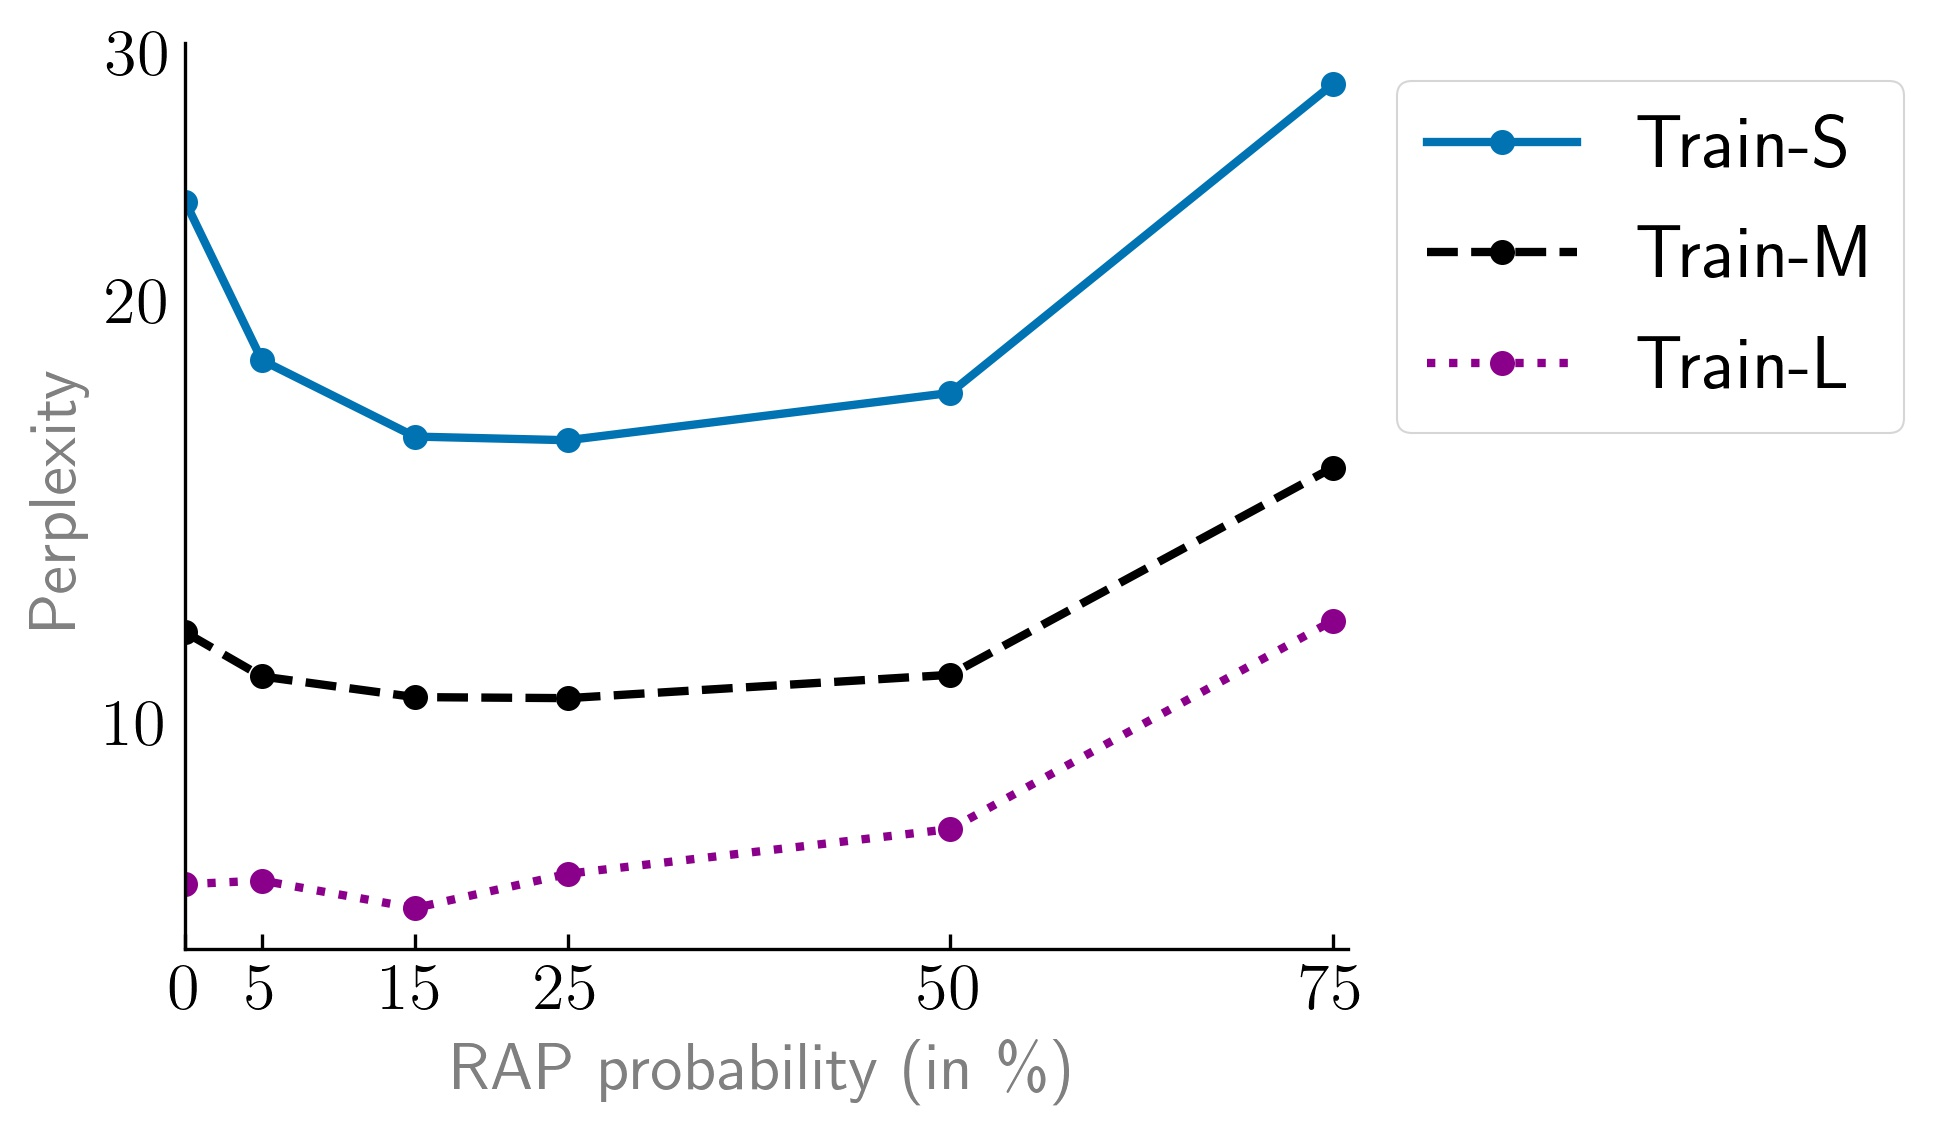
\includegraphics[width=\textwidth]{figures/rap_effect.jpg}
			\captionof{figure}{Validation set perplexities as a function of RAP probabilities for the different training set sizes. RAP $0$ %
				is %
				the standard UCI notation. 
				RAP $100$ is not shown as perplexities are too high. }
			\label{fig:rap_vals}
		\end{minipage}
	\end{minipage}
\end{figure*}

\paragraph{Model Details}
We use the GPT2-small architecture for our base language model \citep{vaswani2017attention,radford2019language}.
GPT2-small is a 12-layer transformer model with 12 attention heads and an embedding size of 768 dimensions.
The context size of the model is limited to 512, which is sufficient to cover the longest game in our training set.
Note that we only borrow the model architecture; the models themselves are \emph{trained from scratch}.
\footnote{Colab notebook to play chess against the base language model \url{https://github.com/shtoshni/learning-chess-blindfolded/blob/master/GPT2_Chess_Model.ipynb}}


For the UCI + RAP $p$ models, we tune over $p \in \{5, 15, 25, 50, 75, 100\}$ based on %
perplexity on the validation set.
Note that for perplexity evaluation, logits corresponding to piece type tokens are masked out since piece type tokens are only available during training.
We find that $p=25$ performs the best for Train-S and Train-M, while $p=15$ is best for Train-L (Figure~\ref{fig:rap_vals}). %
Larger values of $p$ lead to greater mismatch between training and inference, while smaller values likely do not provide enough training signal.

We also experiment with other transformer and non-transformer models in Section~\ref{sec:other_models}.
Among the transformer models, we experiment with two ``approximate" attention models (i.e., models which approximate the full attention of vanilla transformer models), namely, Reformer \cite{kitaev2020reformer} and Performer \cite{choromanski2021rethinking}.  
We set the number of layers and attention heads to 12 for both 
architectures, as in GPT2-small.
We also train LSTM language models with and without RAP. 
For details on hyperparameters and tuning, see Appendix~\ref{sec:hyperparams}.


\paragraph{Training Details}
Models are trained for 10 epochs with a batch size of 60. Validation is performed %
 at the end of every epoch and training stops whenever the validation loss starts increasing.
For optimization we use Adam \citep{kingma2014adam} with learning rate of $5\times10^{-4}$ and L2 weight decay of $0.01$.
The learning rate is warmed up linearly over the first 10\% of training followed by a linear decay.
To accelerate training, we use mixed precision training~\citep{micikevicius2018mixed}. %
All experiments are carried out using the PyTorch Lightning framework %
built on top of PyTorch \citep{falcon2019pytorch, pytorch}.
We use the transformers library \citep{Wolf2019HuggingFacesTS} for all models\footnote{Reformer implementation in \pos{transformers} library is still a work in progress. The presented results are with the 4.2.2 version.} %
except for the Performer model %
for which we use a popular unofficial implementation.
\footnote{\url{https://github.com/lucidrains/performer-pytorch}}








